%-------------------------------------------------------------------------------------------------------
%-------------------------------------------------------------------------------------------------------
%-------------------------------------------------------------------------------------------------------
\subsection{Structure of section}
Every section of this chapter is a simulation of the future application. Every simulation is has his own scene (Showed in this document with some images, for example as in Figure: \ref{fig:VREP_scene_example}). This scenes contains the requited quadrotors and targets in order to test the behavior previous real results. Results of vision algorithm is showed in the vrep console(Figure: \ref{fig:Ground_Tracking_VREP_Console}). \\

\begin{figure}[ht]
	\centering
	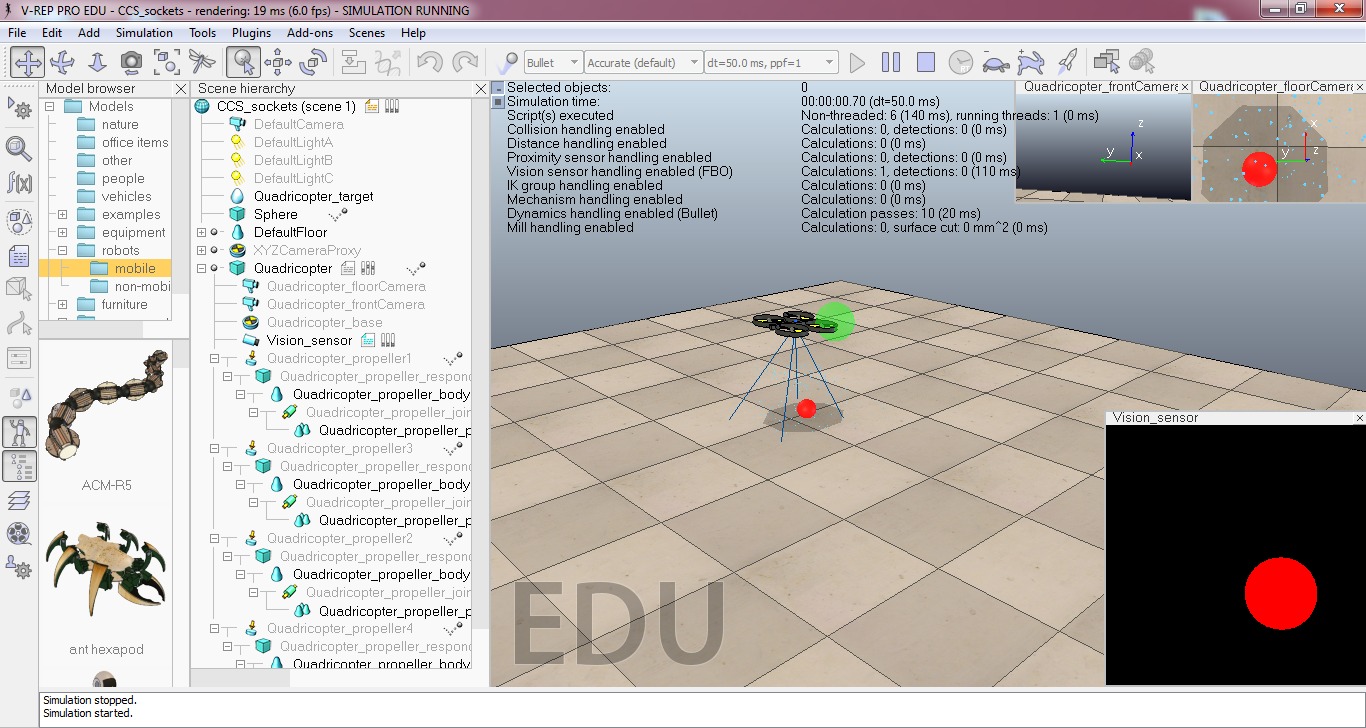
\includegraphics[width=0.8\textwidth,natwidth=1366,natheight=728]{../Images/c3/ground_tracking_scene.png}
	\caption{Ground Tracking Scene}
	\label{fig:VREP_scene_example}
\end{figure}

\begin{figure}[ht]
	\centering
	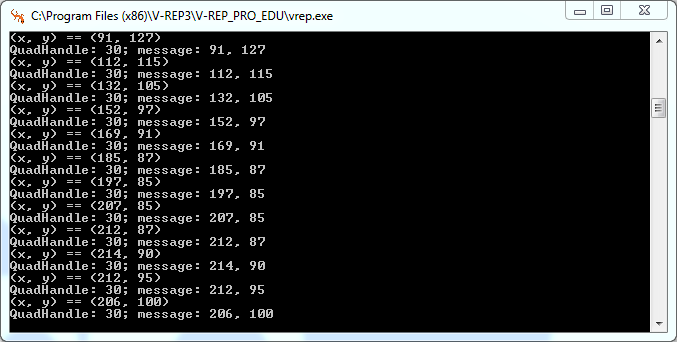
\includegraphics[width=0.8\textwidth,natwidth=677,natheight=342]{../Images/c3/ground_tracking_vrep_console.png}
	\caption{Ground Tracking V-REP Console}
	\label{fig:Ground_Tracking_VREP_Console}
\end{figure}

There is another component in the simulations, the ground station, with the aim to make the most realistic simulations, this ground station is exactly the same as real test ground station. This is possible due to the abstraction of the communication through sockets. The ground station has a simple interface to get some information about the progress. An example of this interface is shown in the Figure: \ref{fig:Ground_Tracking_Server_Console}.

\begin{figure}[ht]
	\centering
	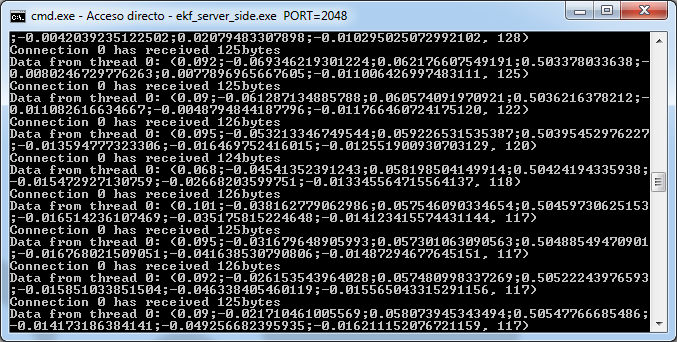
\includegraphics[width=0.8\textwidth,natwidth=677,natheight=342]{../Images/c3/ground_tracking_server_console.png}
	\caption{Ground Tracking Server Console}
	\label{fig:Ground_Tracking_Server_Console}
\end{figure}

Both ground station and objects in the simulation generate a LOG in order to analyze afterwards the results.

%-------------------------------------------------------------------------------------------------------
%-------------------------------------------------------------------------------------------------------
%-------------------------------------------------------------------------------------------------------
\subsection{Simulation 1 - Simple ground camera tracking. Vertical camera}
\subsubsection{Set up}
This Scene has basically one quad rotor and one target (Figure: \ref{fig:VREP_scene_example}). The Red sphere is moving on the floor (Describing a circle) while the quad's camera captures pictures and the on board (simulated) computer process it and command the drone in order to follow the target. In this simulation the camera is facing the ground (Figure: \ref{fig:ground_tracking_scene_vertical}).

\begin{figure}[ht]
	\centering
	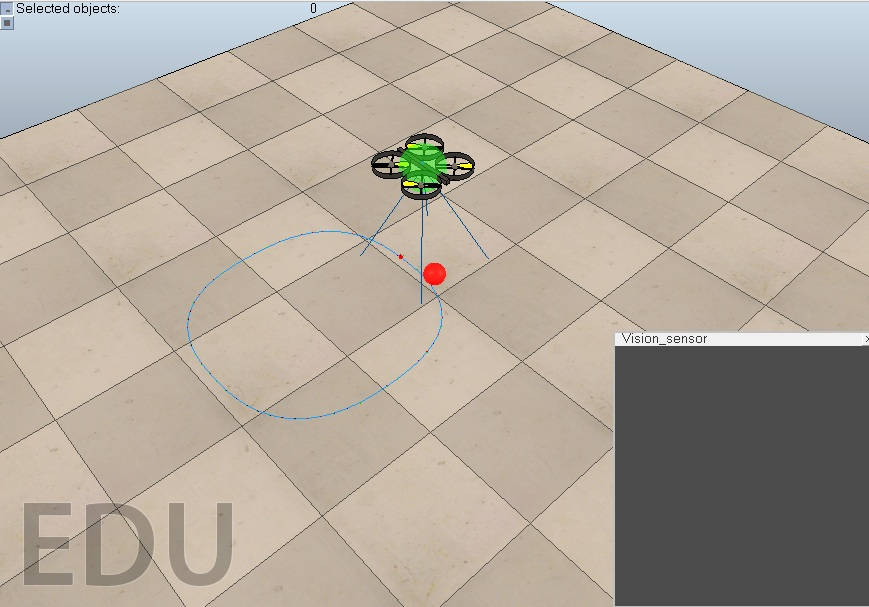
\includegraphics[width=0.65\linewidth]{../Images/c3/ground_tracking_scene_vertical}
	\caption{Ground tracking - Oblique Camera}
	\label{fig:ground_tracking_scene_vertical}
\end{figure}

\subsubsection{Test and results}

	In this test the maximum error (That is about 1 cm) is at the beginning of the simulation Due to the initial state of the EKF. Lately the this error is reduced to $\sim$ 0. The fist figure (\ref{fig:sim1_traj_ori} and \ref{fig:sim1_traj_track}) that contains 2 pictures, shows X and Y coordinate of the a) real trajectory and b) the results of EKF algorithm. The last figure of this simulation shows the 3D path that was described by the target (Blue line) and the tracked trajectory (Red line); Figure \ref{fig:sim1_traj_both_3d}.
	
\begin{figure}[htp]
	\centering
	\begin{subfigure}{0.45\linewidth}
		\centering
		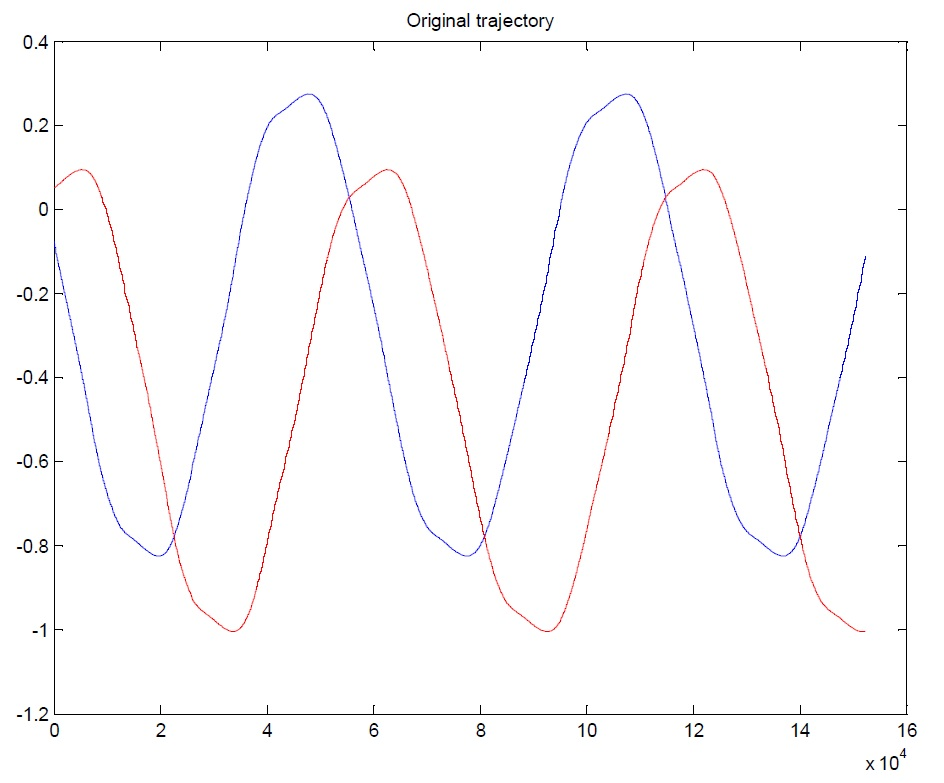
\includegraphics[width=\linewidth]{../Images/c3/sim1_traj_ori}
		\caption{Ground tracking - Original trajectory}
		\label{fig:sim1_traj_ori}
	\end{subfigure}
	~
	\begin{subfigure}{0.45\linewidth}
		\centering
		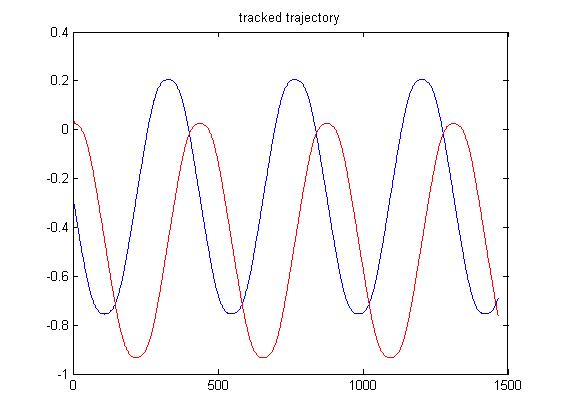
\includegraphics[width=\linewidth]{../Images/c3/sim1_traj_track}
		\caption{Ground tracking - Tracked trajectory}
		\label{fig:sim1_traj_track}
	\end{subfigure}

\end{figure}


\begin{figure}[ht]
\centering
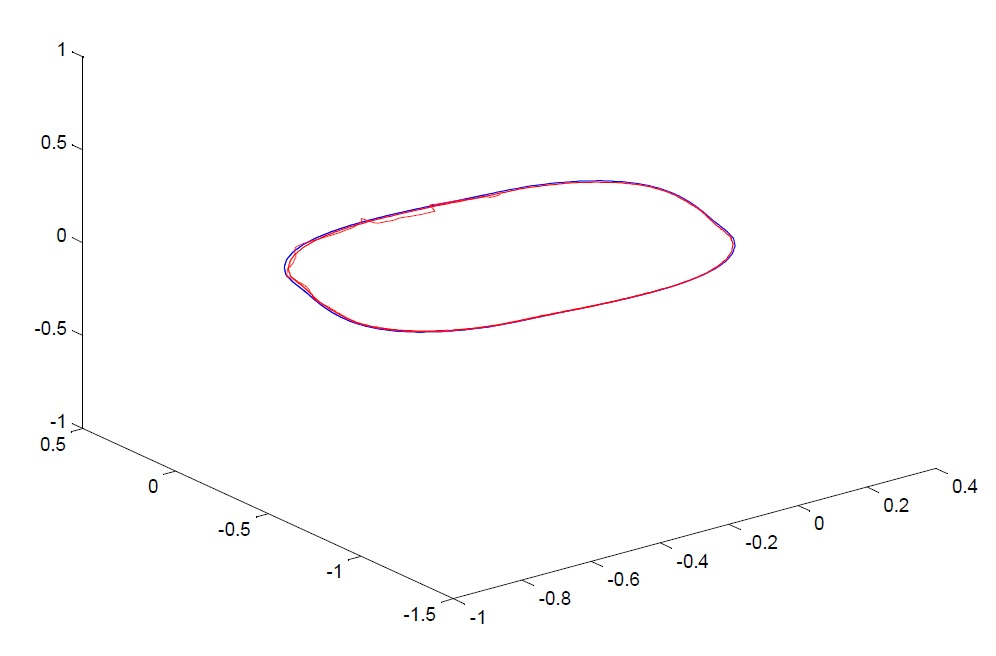
\includegraphics[width=0.7\linewidth]{../Images/c3/sim1_traj_both_3d}
\caption{Ground tracking - Oblique Camera - 3D trajectory}
\label{fig:sim1_traj_both_3d}
\end{figure}




%-------------------------------------------------------------------------------------------------------
%-------------------------------------------------------------------------------------------------------
%-------------------------------------------------------------------------------------------------------
\subsection{Simulation 2 - Simple ground camera tracking. Oblique camera}
\subsubsection{Set up}
This Scene has basically one quad rotor and one target. The Red sphere is moving on the floor (Describing a curve) while the quad's camera captures pictures and the on board (simulated) computer process it and command the drone in order to follow the target. In this case, the camera is not facing directly the ground, now it's oblique (45 degrees from the previous; Figure: \ref{fig:ground_tracking_scene_oblique}). At this experiment, the speed of the target was increased.

\begin{figure}[hp]
	\centering
	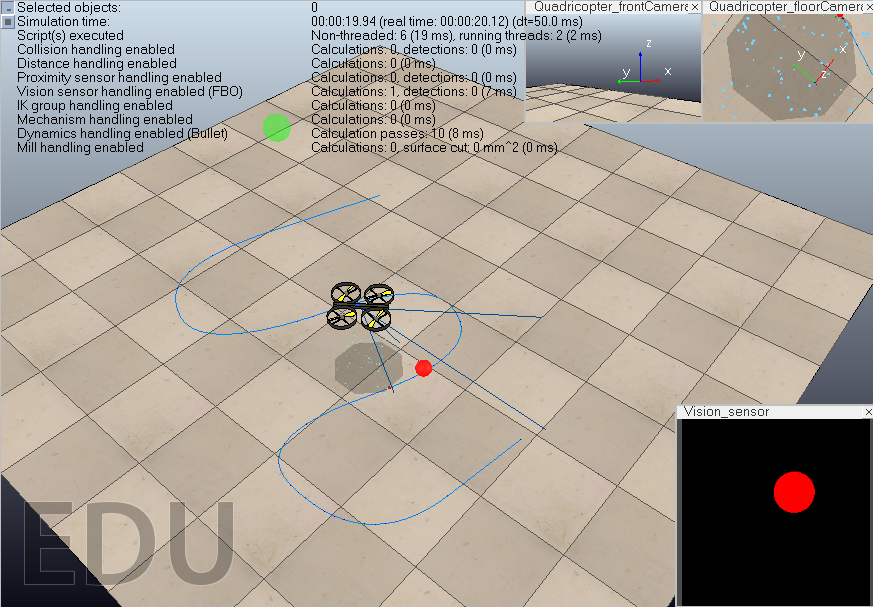
\includegraphics[width=0.65\linewidth]{../Images/c3/ground_tracking_scene_oblique}
	\caption{Ground tracking - Oblique Camera}
	\label{fig:ground_tracking_scene_oblique}
\end{figure}

\subsubsection{Test and results}
\label{lab:sim2_test_results}
In this test the maximum error, apart from the beginning that is large initially due to the initial state of EKF until it's established, is $\sim$ 2 cm due to the speediness of the target at the curve. Lately the this error is reduced to $\sim$ 0. The fist figure (\ref{fig:sim2_traj_ori} and \ref{fig:sim2_traj_track}) that contains 2 pictures, shows X and Y coordinate of the a) real trajectory and b) the results of EKF algorithm. The last figure of this simulation shows the 3D path that was described by the target (Blue line) and the tracked trajectory (Red line); Figure \ref{fig:sim2_traj_both_3d}.

\begin{figure}[htp]
	\centering
	\begin{subfigure}[htp]{0.48\linewidth}
		\centering
		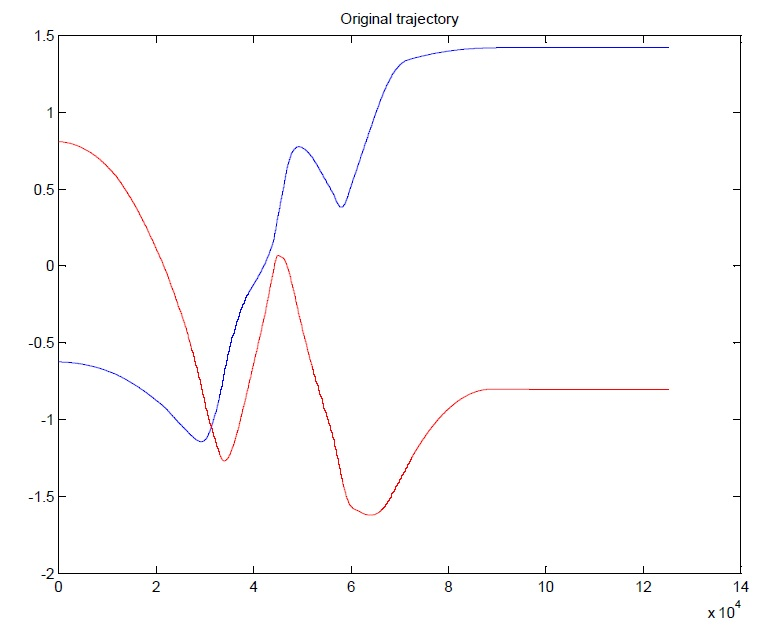
\includegraphics[width=\linewidth]{../Images/c3/sim2_traj_ori}
		\caption{Ground tracking - Original trajectory}
		\label{fig:sim2_traj_ori}
	\end{subfigure}
	~
	\begin{subfigure}[htp]{0.48\linewidth}
		\centering
		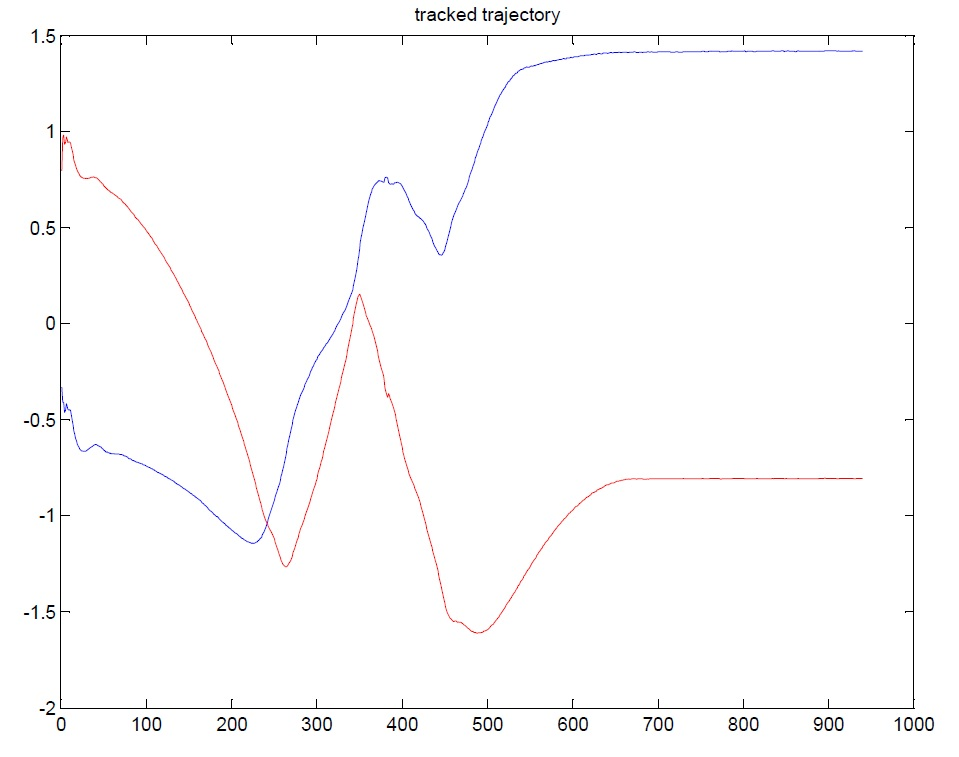
\includegraphics[width=\linewidth]{../Images/c3/sim2_traj_track}
		\caption{Ground tracking - Tracked trajectory}
		\label{fig:sim2_traj_track}
	\end{subfigure}

\end{figure}


\begin{figure}[h]
\centering
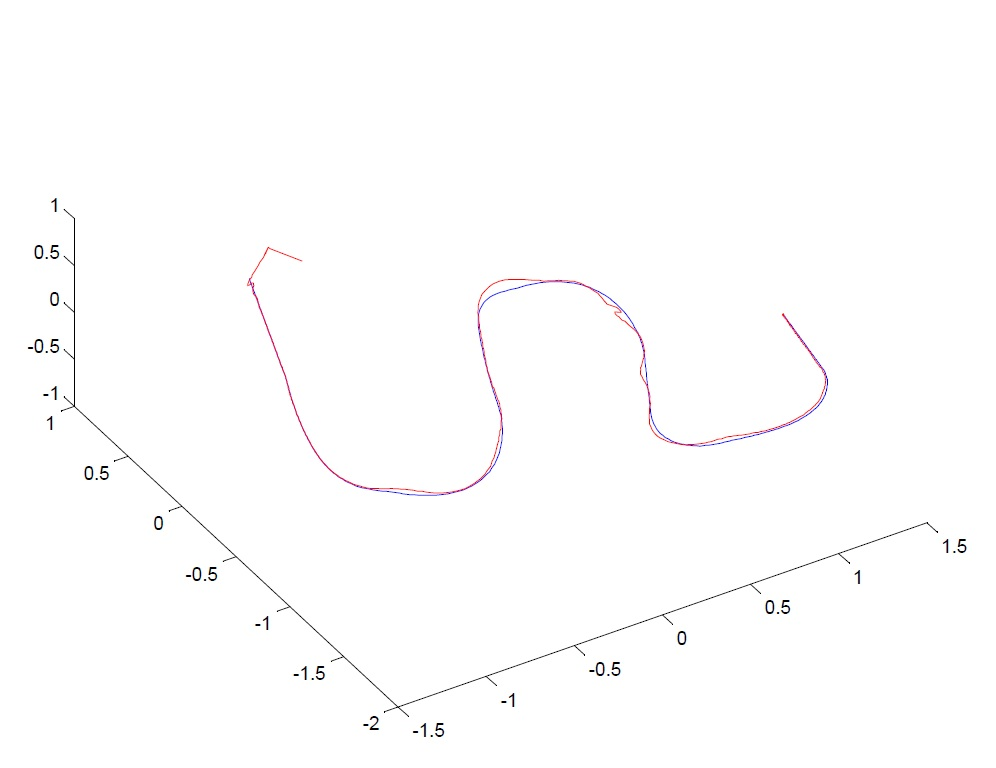
\includegraphics[width=0.9\linewidth]{../Images/c3/sim2_traj_both_3d}
\caption{Ground tracking - Oblique Camera - 3D trajectory}
\label{fig:sim2_traj_both_3d}
\end{figure}




%-------------------------------------------------------------------------------------------------------
%-------------------------------------------------------------------------------------------------------
%-------------------------------------------------------------------------------------------------------
\subsection{Simulation 3 - Stereo tracking}
\subsubsection{Set up}
This simulation is the first one with two quadcopters. The Red sphere is moving on the floor (Describing a curve) while both quad's cameras capture pictures and the on board computers (that are simulated) process them and self-command quads in order to follow the target. The cameras are also oblique (45 degrees from the previous; Figure: \ref{fig:sim3_set_up}). The speediness is the same one that in simulation 2.


\begin{figure}[htp]
	\centering
	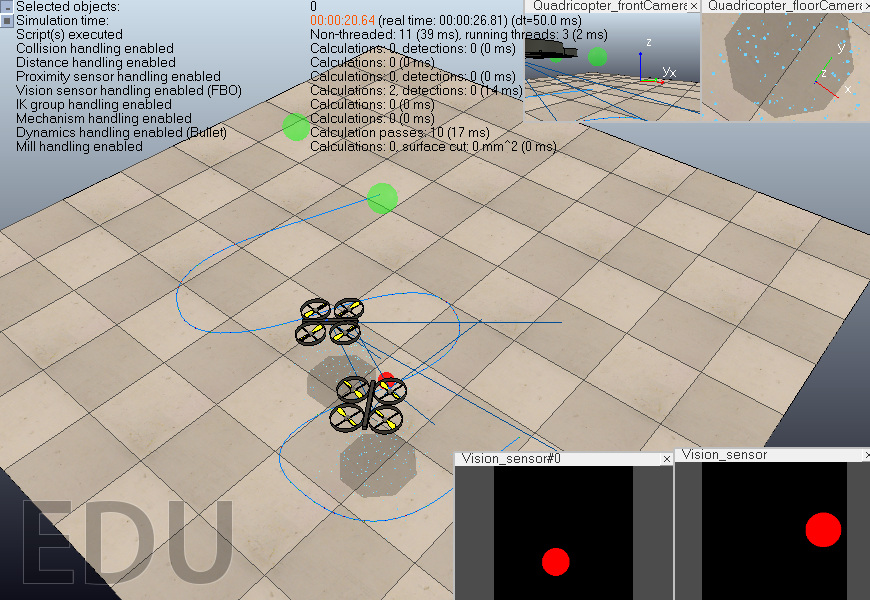
\includegraphics[width=0.65\linewidth]{../Images/c3/sim3_set_up}
	\caption{Stereo tracking - Set up}
	\label{fig:sim3_set_up}
\end{figure}


%\begin{figure}[h]
%	\centering
%	\begin{subfigure}[b]{0.4\linewidth}
%	\centering
%		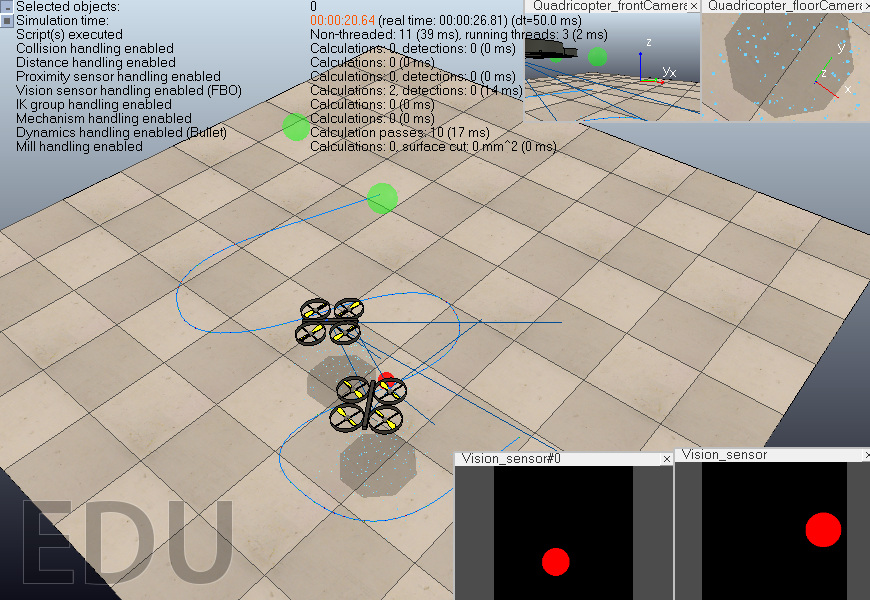
\includegraphics[width=\linewidth]{../Images/c3/sim3_set_up}
%		\caption{Stereo tracking - Set up}
%		\label{fig:sim3_set_up}
%	\end{subfigure}
%	~
%	\begin{subfigure}[b]{0.4\linewidth}
%		\centering
%		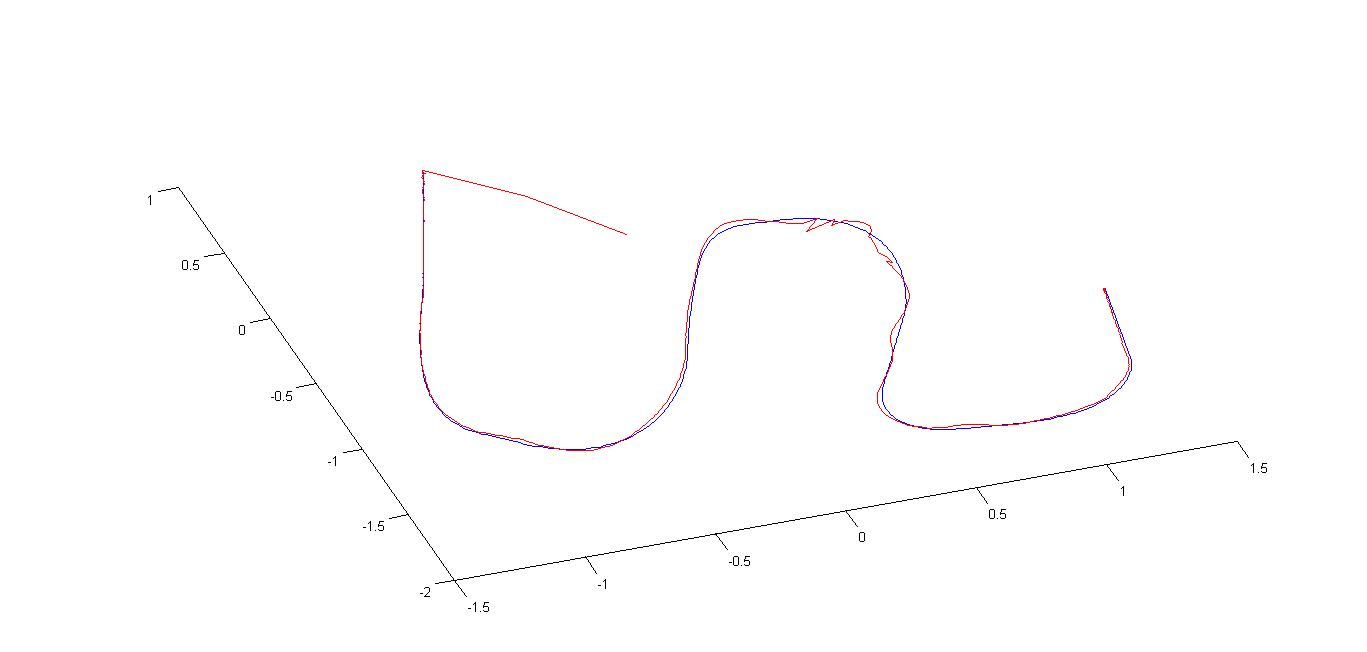
\includegraphics[width=\linewidth]{../Images/c3/sim3_traj_both_3d}
%		\caption{Stereo tracking - 3D trajectory}
%		\label{fig:sim3_traj_both_3d}
%	\end{subfigure}
%\end{figure}

\subsubsection{Test and results}

	In this simulation the results converge fastly from the initial state to the target's position. Here the max error is $\sim$ 3 cm. and medium error is $\sim$ 1 cm. Max error is found at the beginning of the second curve. That is because the target increase it's velocity considerably (And the EKF suppose a linear movement). This, together with the dynamic behavior of the quadrotors, make the path-line seems a sawtooth (Figure: \ref{fig:sim3_traj_both_3d}).
	

\begin{figure}[hp]
	\centering
	\begin{subfigure}[hp]{0.48\linewidth}
		\centering
		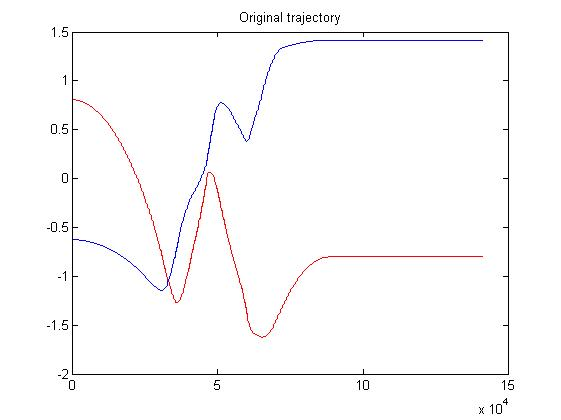
\includegraphics[width=\linewidth]{../Images/c3/sim3_traj_ori}
		\caption{Stereo tracking - Original trajectory}
		\label{fig:sim3_traj_ori}
	\end{subfigure}
	~
	\begin{subfigure}[hp]{0.48\linewidth}
		\centering
		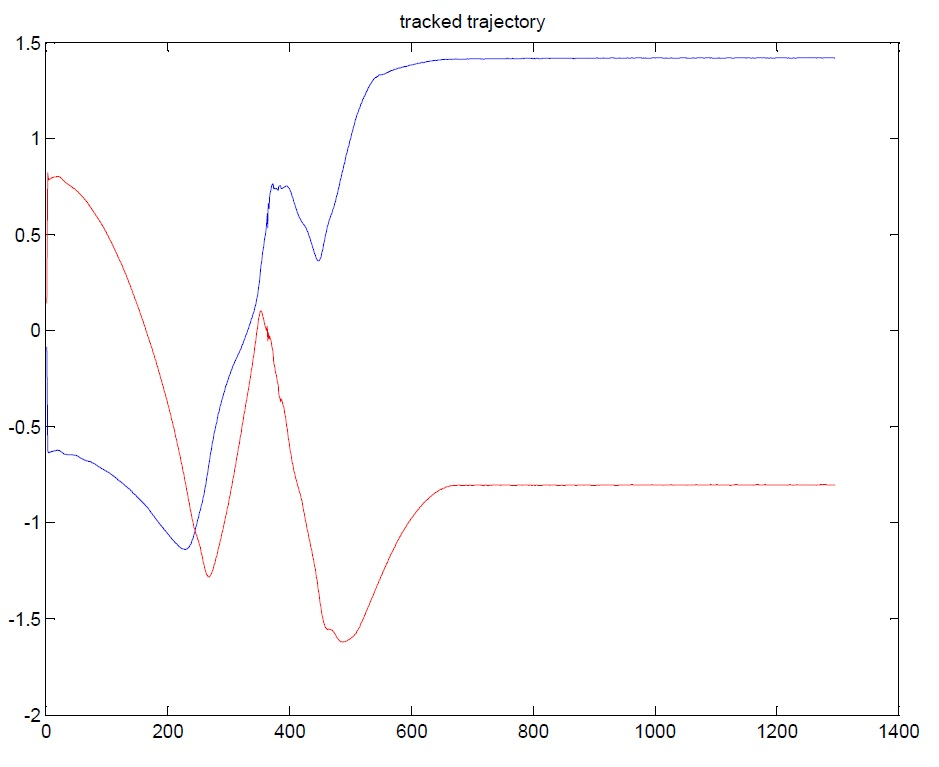
\includegraphics[width=\linewidth]{../Images/c3/sim3_traj_track}
		\caption{Stereo tracking - Tracked trajectory}
		\label{fig:sim3_traj_track}
	\end{subfigure}
\end{figure}

\begin{figure}[htp]
		\centering
		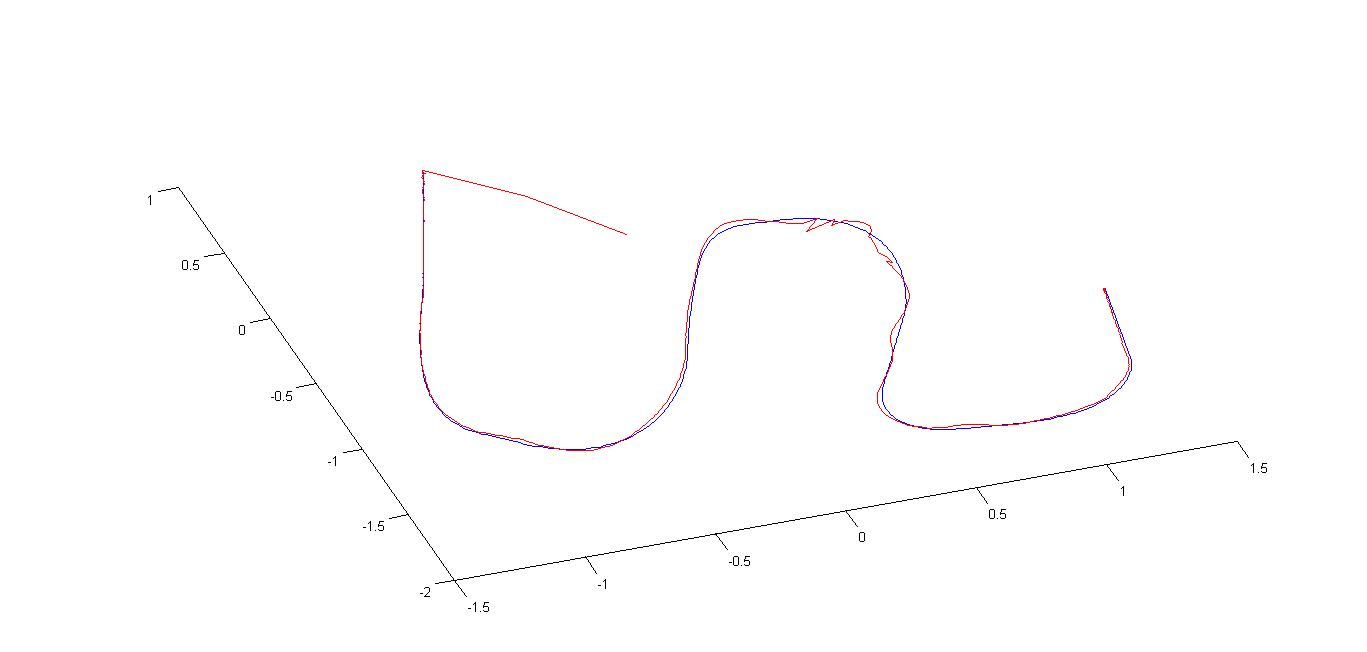
\includegraphics[width=0.7\linewidth]{../Images/c3/sim3_traj_both_3d}
		\caption{Stereo tracking - 3D trajectory}
		\label{fig:sim3_traj_both_3d}
\end{figure}

%-------------------------------------------------------------------------------------------------------
%-------------------------------------------------------------------------------------------------------
%-------------------------------------------------------------------------------------------------------
\subsection{Simulation 4 - Ground Tracking, Multiple targets}
\subsubsection{Set up}
 On this experiment, there is again only one quadrotor(Figure: \ref{fig:sim4_set_up}). Instead, one more target was added (Blue sphere). Both objects describe the curve, keeping their relative distance (Moving as a rigid solid, so the blue is always on the left-side of the path). the watcher's camera is also oblique (45 degrees) and spheres keeps the same speed of the previous simulation.
 
\begin{figure}[htp]
	\centering
	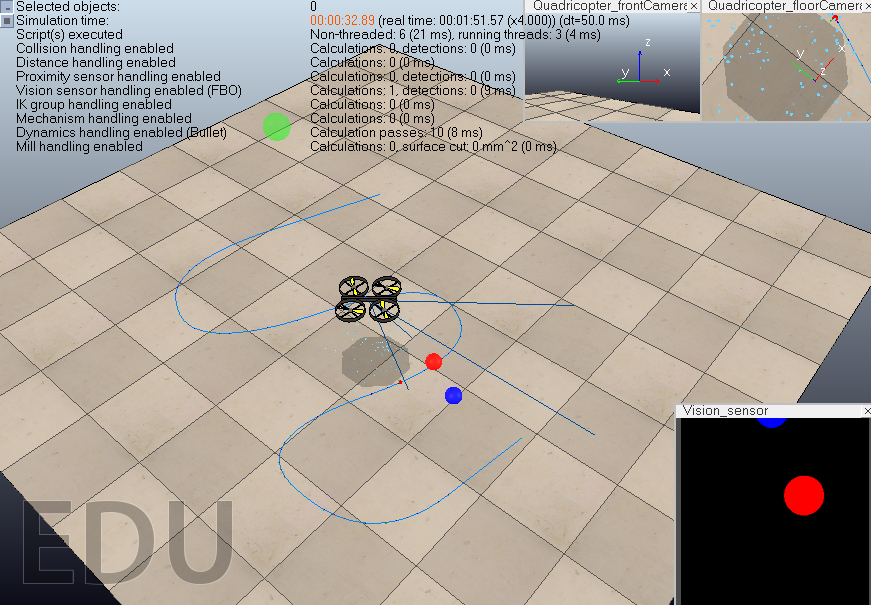
\includegraphics[width=0.6\linewidth]{../Images/c3/sim4_set_up}
	\caption{Multiple Targets - Set Up}
	\label{fig:sim4_set_up}
\end{figure}

\subsubsection{Test and results}

	Firstly, figures \ref{fig:sim4_redtarget} and \ref{fig:sim4_bluetarget} shows the X and Y coordinate of the targets (Both real and estimate). Secondly, figure \ref{fig:sim4_3dtraj} shows the 3D path-lines of both red and blue spheres. \\
	
	\begin{figure}[hp]
		\centering
		\begin{subfigure}[hp]{0.45\linewidth}
			\centering
			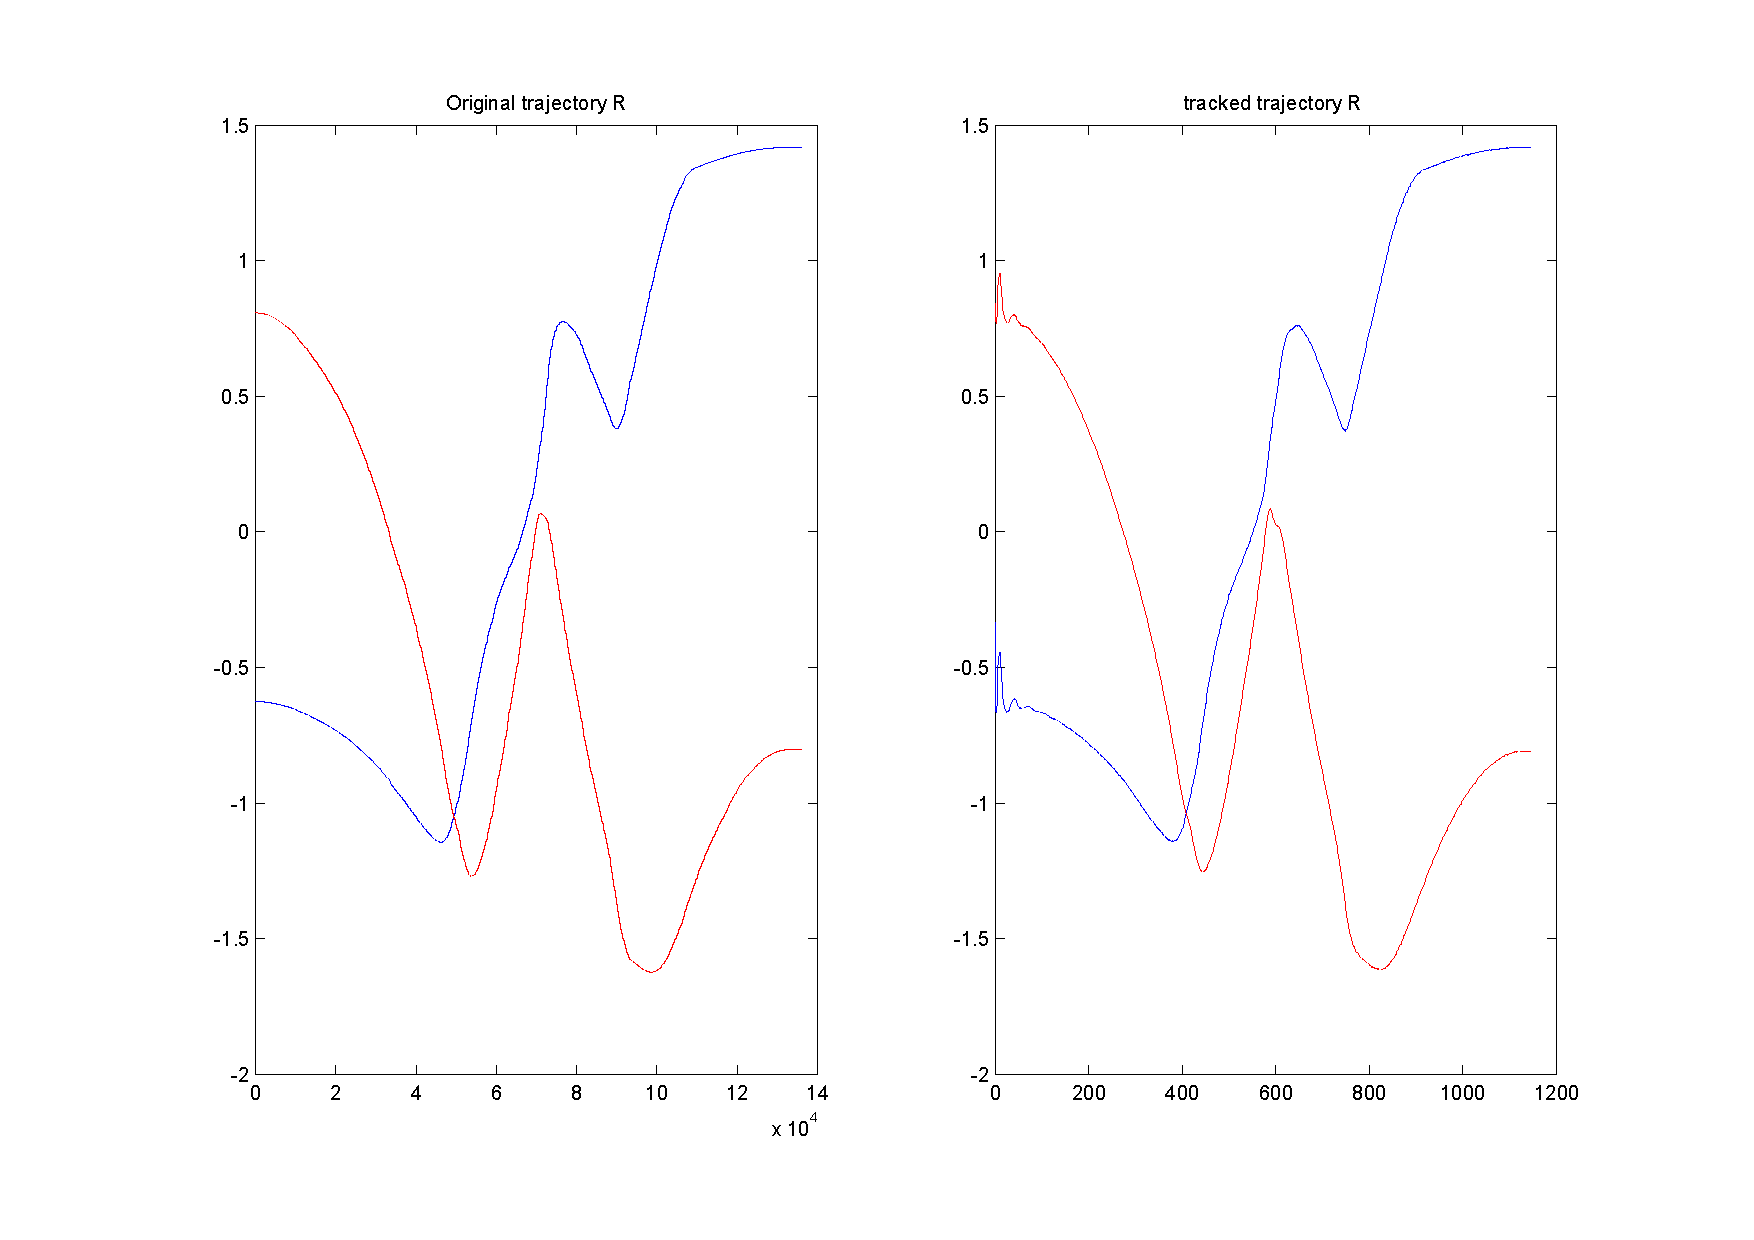
\includegraphics[width=\linewidth]{../Images/c3/sim4_redtarget}
			\caption{Multiple Targets - Red target}
			\label{fig:sim4_redtarget}	
		\end{subfigure}
		~
		\begin{subfigure}[hp]{0.45\linewidth}
			\centering
			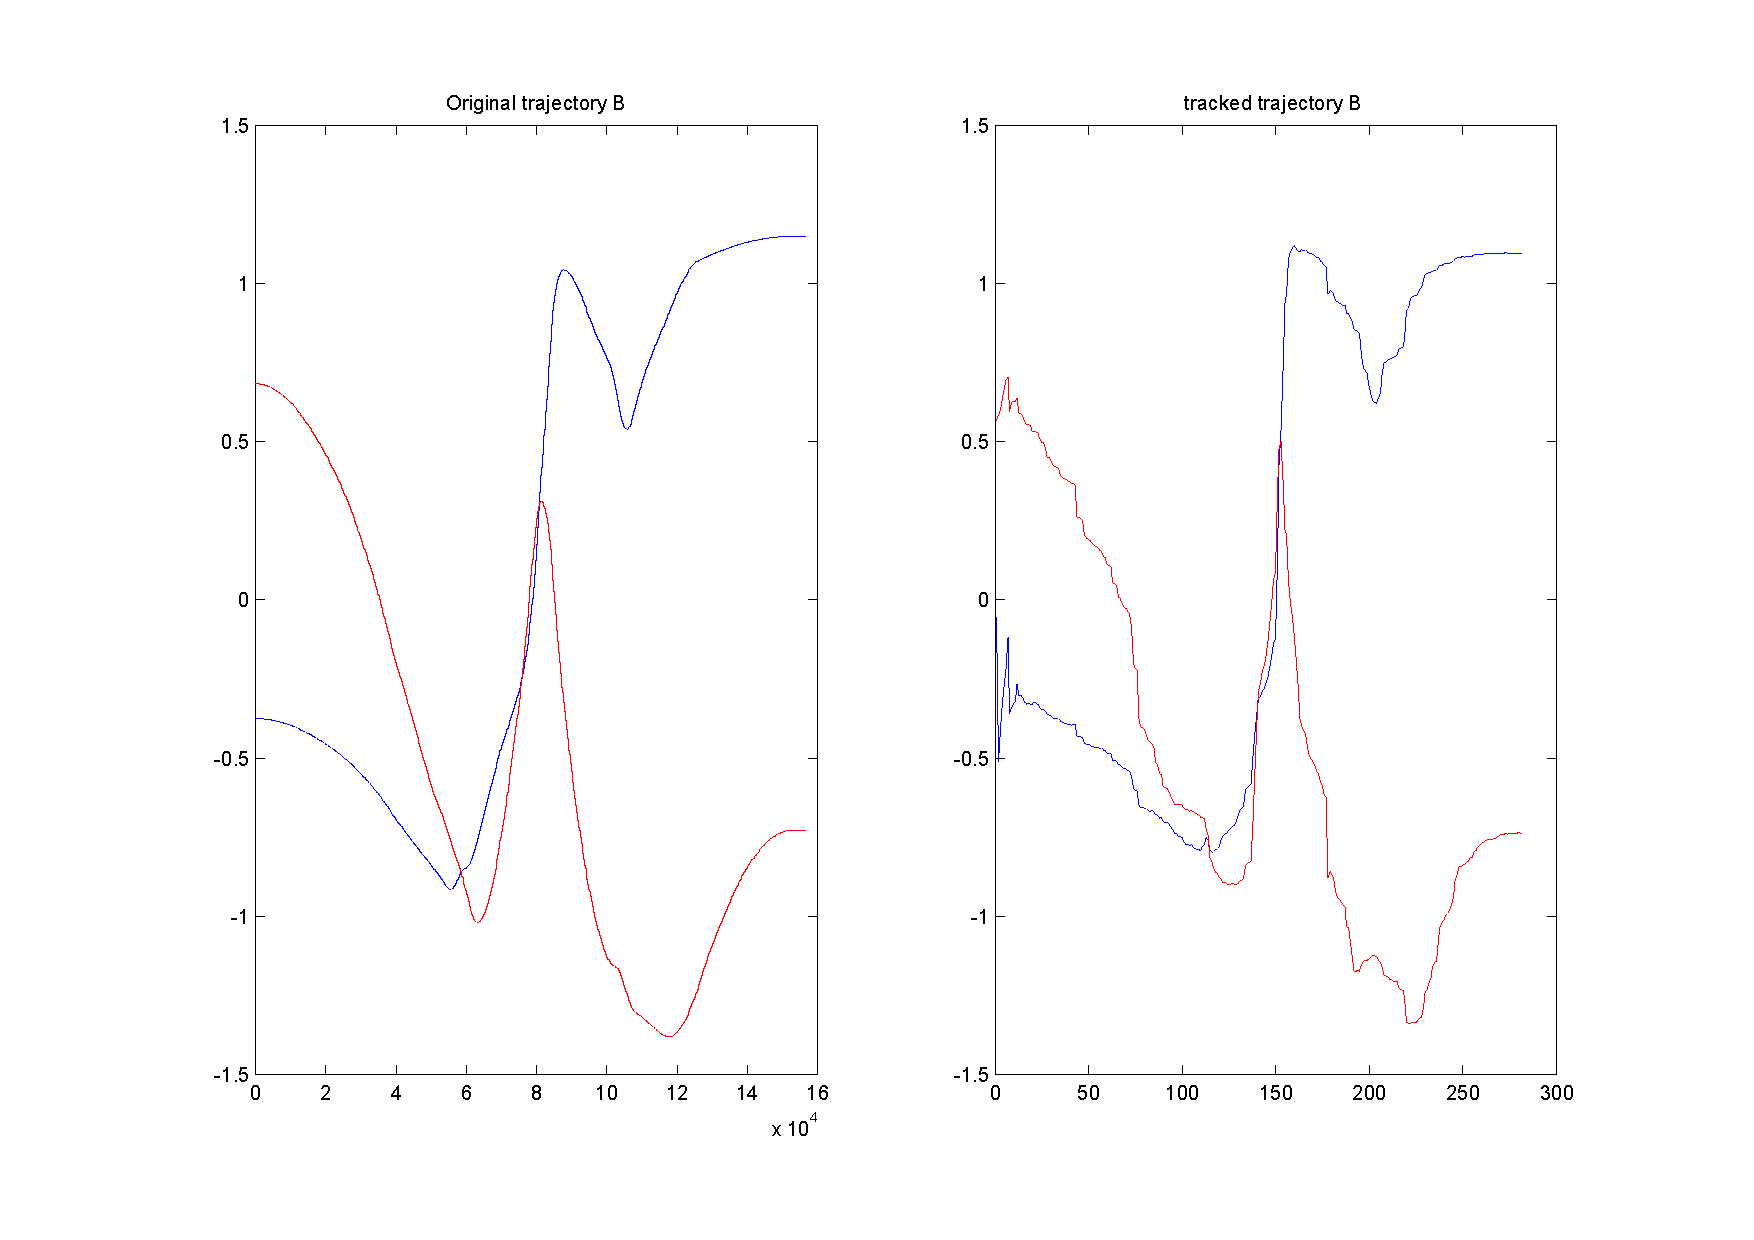
\includegraphics[width=\linewidth]{../Images/c3/sim4_bluetarget}
			\caption{Multiple Targets - Blue target}
			\label{fig:sim4_bluetarget}
		\end{subfigure}
	\end{figure}
	
	The results of red tracking are quite good and similar to the ones explained in "Ground tracking - Oblique camera" \ref{fig:sim2_traj_both_3d}. The tracking of the blue sphere seems to be wrong. However, it is not. This deviation is due to lack of information. The camera didn't capture the whole blue sphere \ref{fig:sim4_centroid_objs}, causing an error between the centroid of the recognized part of the sphere in the image and the real one. That's why the tracked-path is always displaced a few centimeters from the real one. The maximum error is $\sim$ 15 cm and the medium is $\sim$ 6 cm.



\begin{figure}[hp]
	\centering
	\begin{subfigure}{0.45\linewidth}
		\centering
		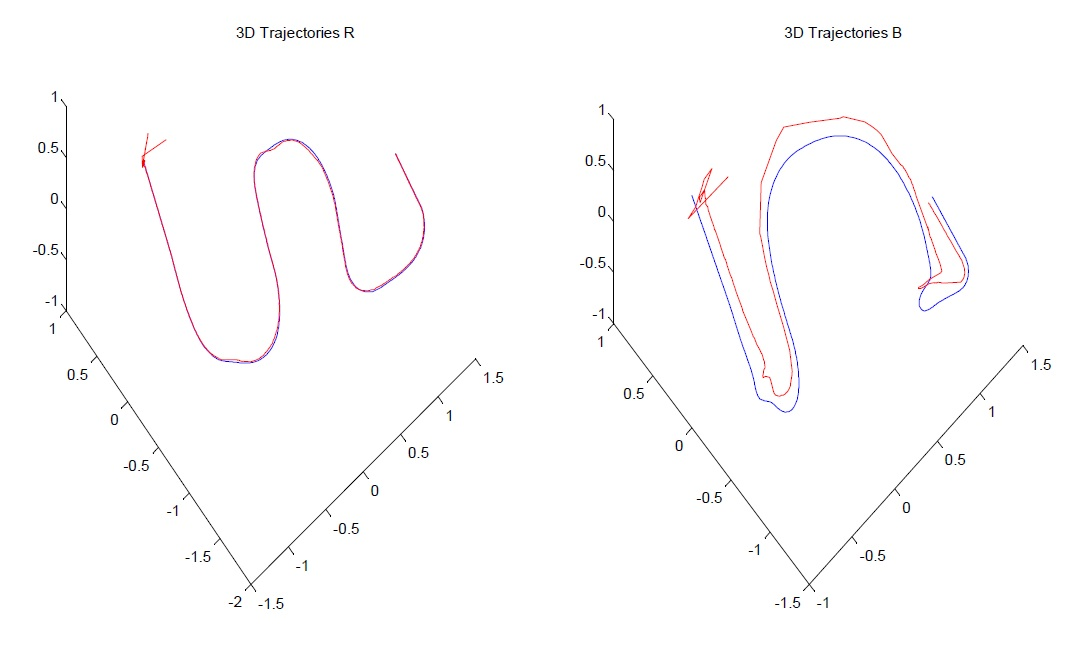
\includegraphics[width=\linewidth]{../Images/c3/sim4_3dtraj}
		\caption{Multiple Targets - 3D trajectory}
		\label{fig:sim4_3dtraj}
	\end{subfigure}
	~
	\begin{subfigure}{0.2\linewidth}
		\centering
		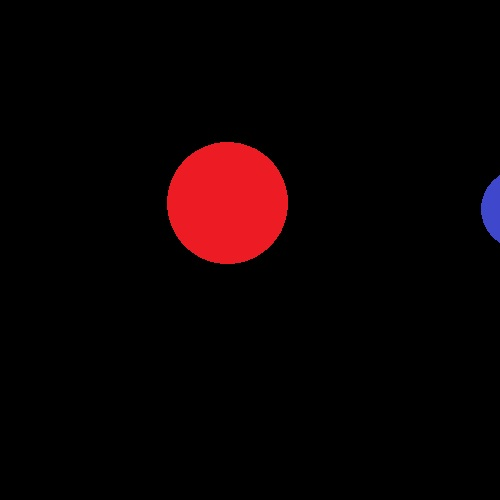
\includegraphics[width=\linewidth]{../Images/c3/sims_two_object_centroid_out}
		\caption{Multiple Targets - Objects centroids on Image}
		\label{fig:sim4_centroid_objs}
	\end{subfigure}
\end{figure}